\documentclass{beamer}

\mode<presentation> {
	
	% The Beamer class comes with a number of default slide themes
	% which change the colors and layouts of slides. Below this is a list
	% of all the themes, uncomment each in turn to see what they look like.
	
	%\usetheme{default}
	%\usetheme{AnnArbor}
	%\usetheme{Antibes}
	%\usetheme{Bergen}
	%\usetheme{Berkeley}
	%\usetheme{Berlin}
	%\usetheme{Boadilla}
	%\usetheme{CambridgeUS}
	%\usetheme{Copenhagen}
	%\usetheme{Darmstadt}
	%\usetheme{Dresden}
	%\usetheme{Frankfurt}
	%\usetheme{Goettingen}
	%\usetheme{Hannover}
	%\usetheme{Ilmenau}
	%\usetheme{JuanLesPins}
	%\usetheme{Luebeck}
	\usetheme{Madrid}
	%\usetheme{Malmoe}
	%\usetheme{Marburg}
	%\usetheme{Montpellier}
	%\usetheme{PaloAlto}
	%\usetheme{Pittsburgh}
	%\usetheme{Rochester}
	%\usetheme{Singapore}
	%\usetheme{Szeged}
	%\usetheme{Warsaw}
	
	% As well as themes, the Beamer class has a number of color themes
	% for any slide theme. Uncomment each of these in turn to see how it
	% changes the colors of your current slide theme.
	
	%\usecolortheme{albatross}
	%\usecolortheme{beaver}
	%\usecolortheme{beetle}
	%\usecolortheme{crane}
	%\usecolortheme{dolphin}
	%\usecolortheme{dove}
	%\usecolortheme{fly}
	%\usecolortheme{lily}
	%\usecolortheme{orchid}
	%\usecolortheme{rose}
	%\usecolortheme{seagull}
	%\usecolortheme{seahorse}
	%\usecolortheme{whale}
	%\usecolortheme{wolverine}
	
	%\setbeamertemplate{footline} % To remove the footer line in all slides uncomment this line
	%\setbeamertemplate{footline}[page number] % To replace the footer line in all slides with a simple slide count uncomment this line
	
	%\setbeamertemplate{navigation symbols}{} % To remove the navigation symbols from the bottom of all slides uncomment this line
}

\usepackage{graphicx} % Allows including images
\usepackage{booktabs} % Allows the use of \toprule, \midrule and \bottomrule in tables 

\usepackage[T1]{fontenc}
\usepackage[utf8]{inputenc}
\setbeamertemplate{caption}[numbered]
\newcommand{\C}{\mathbb{C}}
\newcommand{\R}{\mathbb{R}}
\newcommand{\Q}{\mathbb{Q}}
\newcommand{\Z}{\mathbb{Z}}
\newcommand{\N}{\mathbb{N}}
\newcommand{\p}{\mathbb{P}}
\newcommand{\E}{\mathbb{E}}
\usepackage{graphicx}
\usepackage{amssymb}
\usepackage{setspace}
\usepackage[toc,page]{appendix}
\usepackage{epstopdf}
\usepackage{latexsym}
\usepackage{amstext}
\usepackage{lmodern}
\usepackage{amsmath}
\usepackage{bbm}
\usepackage{amsfonts}
\usepackage{url}
\usepackage{bm}
\usepackage{mathrsfs}
\usepackage{mathtools}
\usepackage{float}
%\usepackage{hyperref} give reference hyperlink 
%\usepackage{setspace}
\usepackage{indentfirst}
\usepackage{multirow}
\usepackage{color}
\usepackage{mathtools}
% packages from template
\usepackage{amsmath,amsthm,amssymb,amsfonts}
\usepackage[width=.9\textwidth]{caption}
\usepackage{mathrsfs}
\usepackage{graphicx}
\newcommand{\indep}{\rotatebox[origin=c]{90}{$\models$}}
\usepackage{textgreek}
\usepackage{bbold}
\usepackage{subcaption}
\usepackage{natbib}
\usepackage{verbatim}
\usepackage{soul}
\usepackage[utf8]{inputenc}
\usepackage[algo2e,ruled,vlined]{algorithm2e} 
\usepackage{fancyvrb}


\newtheorem{proposition}[theorem]{Proposition}

\newcommand{\M}{\mathbf{M}}
\newcommand{\rank}{\mathrm{rank}}
\newcommand{\rep}{\mathrm{rep}}
\newcommand{\PR}{\text{Pr}}
\newcommand{\pkg}[1]{{\fontseries{b}\selectfont #1}}
%\newcommand\norm[1]{\left\lVert#1\right\rVert}
\newcommand{\bs}[1]{\boldsymbol{#1}}
\newcommand{\mb}[1]{\mathbf{#1}}
\DeclareMathOperator*{\argmin}{arg\,min}
\DeclarePairedDelimiter{\ceil}{\lceil}{\rceil}
\DeclarePairedDelimiterX{\norm}[1]{\lVert}{\rVert}{#1}
\allowdisplaybreaks
%=============================================================================
% prelude
%=============================================================================
\def\mathLarge#1{\mbox{\LARGE $#1$}}
\usepackage{soul}


\title[]{A Brief Introduction to Survival Analysis}
\author[Hongda Zhang]{Hongda Zhang}
\institute{Nanjing University}
\date{\today}



\begin{document}
	\begin{frame}
		\titlepage
	\end{frame}
	
	\begin{frame}
		\frametitle{Contents}
		\begin{enumerate}
			\item Basic concepts
			\item Kaplan-Meier estimate
			\item Cox regression model
		\end{enumerate}
	\nocite{*}
	\end{frame}

	\begin{frame}
		\frametitle{Basic concepts}
		Survival analysis is a set of statistical methods used to deal with time-to-event problems.
		\begin{itemize}
			\item Survival time (denoted by $t$): the length of time from a starting point to the occurrence of some event of interest. 
			\item Censoring: a survival time is censored if the end-point is not observed. Censored survival time is denoted by $c$.
				\begin{itemize}
					\item right censoring: the actual survival time is greater than that observed.\\
					\item left censoring: the actual survival time is less than that observed.\\
					\item interval censoring: the event happened within an interval.
				\end{itemize}
			\item Independent censoring: the actual survival time is independent from the cause of censoring. Many of the survival analysis methods are not valid without this assumption.
		\end{itemize}
	\end{frame}

	\begin{frame}
		\frametitle{Basic concepts (cont.)}
		\begin{itemize}
			\item The distribution function: let $T$ be the random variable associated with the survival time. Then the distribution of function of $T$ is then given by 
			\[ F( t ) = P( T < t ) = \int_{ 0 }^{ t } f( u ) du,  \]
			which represents the probability of the survival time being less than $t$.
			\item The survivor function:
			\[ S(t) = P( T \geq t ) = 1 - F( t ), \]
			which represents the probability of survival time greater than or equal to $t$.
		\end{itemize}
	\end{frame}

	\begin{frame}
		\frametitle{Basic concepts (cont.)}
		\begin{itemize}
			\item The hazard function: 
			\[ h(t) = \lim_{  \delta \rightarrow 0 }\left\{ \frac{ P( t \leq T < t + \delta | T \geq t ) }{ \delta } \right\}, \]
			which represents a instantaneous event rate at time $t$. 
			(Note: $ h( t ) = \frac{ f( t ) }{ S( t ) }$)
			\item The cumulative hazard function:
			\[ H( t ) = \int_{ 0 }^{ t } h( u ) du, \]
			represents the cumulative risk of an event happening by time $t$.
			(Note: $H( t ) = - \log S( t )$.) 
		\end{itemize}
	\end{frame}
	
	\begin{frame}
		\frametitle{Kaplan-Meier estimate of the survivor function}
		Suppose there are $n$ individuals with the corresponding survival times $t_1, t_2, \dots, t_n$. Let the $r$ distinct survival times be order as $t_{ ( 1 ) } < t_{ ( 2 ) } < \dots < t_{ ( r ) }$. Let $n_j$ denote the number of individuals alive right before $t_{ ( j ) }$ and $d_{ ( j ) }$ denote the number of event (death) at time $t_{ ( j ) }$. Then the Kaplan-Meier estimate of the survivor function is given by
		\[ \hat{ S }( t ) = \prod_{ j = 1 }^{ k } \frac{ n_j - d_j }{ n_j }, \]
		for $t_{ ( k ) } \leq t < t_{ ( k + 1 ) }$, $k = 1, 2, \dots, r$, with $\hat{ S }( t ) = 1$ for $t < t_{ ( 1 ) }$ and $ t_{ ( r + 1 ) } = \infty$.
			
	\end{frame}
	
	\begin{frame}
		\frametitle{Kaplan-Meier estimate of the survivor function (cont.)}
		\framesubtitle{Standard error of the estimated survivor function}
		The Kaplan-Meier estimate of the survivor function can be rewritten as 
		\[ \hat{ S }( t ) = \prod_{ j = 1 }^{ k } \hat{ p }_j, \]
		for $t_{ ( k ) } \leq t < t_{ ( k + 1 ) }$, $k = 1, 2, \dots, r$, where $\hat{ p } = \frac{ n_j - d_j }{ n_j }$.
		\begin{align*}
			\log \hat{ S }( t ) & = \sum_{ j = 1 }^{ k } \log \hat{ p }_j \\
			\text{var}\left\{ \log \hat{ S }( t ) \right\} & = \sum_{ j = 1 }^{ k } \text{var} \{ \log \hat{ p }_j \}
		\end{align*}
	\end{frame}

	\begin{frame}
		\frametitle{Kaplan-Meier estimate of the survivor function (cont.)}
		\framesubtitle{Standard error of the estimated survivor function}
		It can be shown that 
		\[ \text{se}\left\{ \hat{ S }( t ) \right\} \approx \hat{ S }( t ) \left\{ \sum_{ j = 1 }^{ k } \frac{ d_j }{ n_j ( n_j - d_j ) }  \right\} ^ \frac{ 1 }{ 2 }, \]
		for $t_{ ( k ) } \leq t < t_{ ( k + 1 ) }$.
	\end{frame}

	\begin{frame}
		\frametitle{Kaplan-Meier estimate of the survivor function (cont.)}
		\framesubtitle{Confidence intervals for the values of survivor function}
		With the assumption that the estimated value of the survivor function at $t$ is normally distributed with mean $S( t )$ and estimated standard error $\text{se}\left\{ \hat{ S }( t ) \right\}$, then a $100( 1 - \alpha)\%$ confidence interval for $S( t )$ is given by
		\[ \left( \hat{ S }( t ) - z_{ \alpha / 2 } \text{se}\left\{ \hat{ S }( t ) \right\}, \hat{ S }( t ) + z_{ \alpha / 2 } \text{se}\left\{ \hat{ S }( t ) \right\} \right), \]
		where $z_{ \alpha / 2 }$ is the $( 1 - \alpha / 2 )$th percentile of standard normal distribution.
	\end{frame}
	
	\begin{frame}[fragile]
		\frametitle{Kaplan-Meier estimate of the survivor function (cont.)}
		\framesubtitle{An example}
		Now use the lung cancer data in \texttt{survival} package of R as an example.
		The code below loads \texttt{survival} and \texttt{survminer} packages and shows the information of of lung dataset.
		\begin{Verbatim}
> ###########################################
> ## Examples of survival analysis using R ##
> ###########################################
> 
> library( survival )
> library( survminer )
> ?lung
		\end{Verbatim}
	\end{frame}
	
		\begin{frame}[fragile]
		\frametitle{Kaplan-Meier estimate of the survivor function (cont.)}
		\framesubtitle{An example}
		The format of the lung dataset is show below:
		\begin{Verbatim}[fontsize=\small]
inst:      Institution code
time:      Survival time in days
status:    censoring status 1=censored, 2=dead
age:       Age in years
sex:       Male=1 Female=2
ph.ecog:   ECOG performance score as rated by the physician. 
           0=asymptomatic, 1= symptomatic but completely
           ambulatory, 2= in bed <50% of the day, 3= in bed > 50% 
           of the day but not bedbound, 4 = bedbound
ph.karno:  Karnofsky performance score (bad=0-good=100) rated by 
           physician
pat.karno: Karnofsky performance score as rated by patient
meal.cal:  Calories consumed at meals
wt.loss:   Weight loss in last six months (pounds)
		\end{Verbatim}
	\end{frame}
	\begin{frame}[fragile]
		\frametitle{Kaplan-Meier estimate of the survivor function (cont.)}
		\framesubtitle{An example}
		Then run the code below to get and plot the Kaplan-Meier estimate of the survivor function. 
		\begin{Verbatim}[fontsize=\small]
## Kaplan-Meier estimate 
km <- survfit( Surv( time, status ) ~ 1, data = lung )
## Generate graphs
ggsurvplot( km_sex )
		\end{Verbatim}
	\end{frame}
	
	\begin{frame}
		\frametitle{Kaplan-Meier estimate of the survivor function (cont.)}
		\framesubtitle{An example}
		
		\begin{figure}[H]
			\centering
			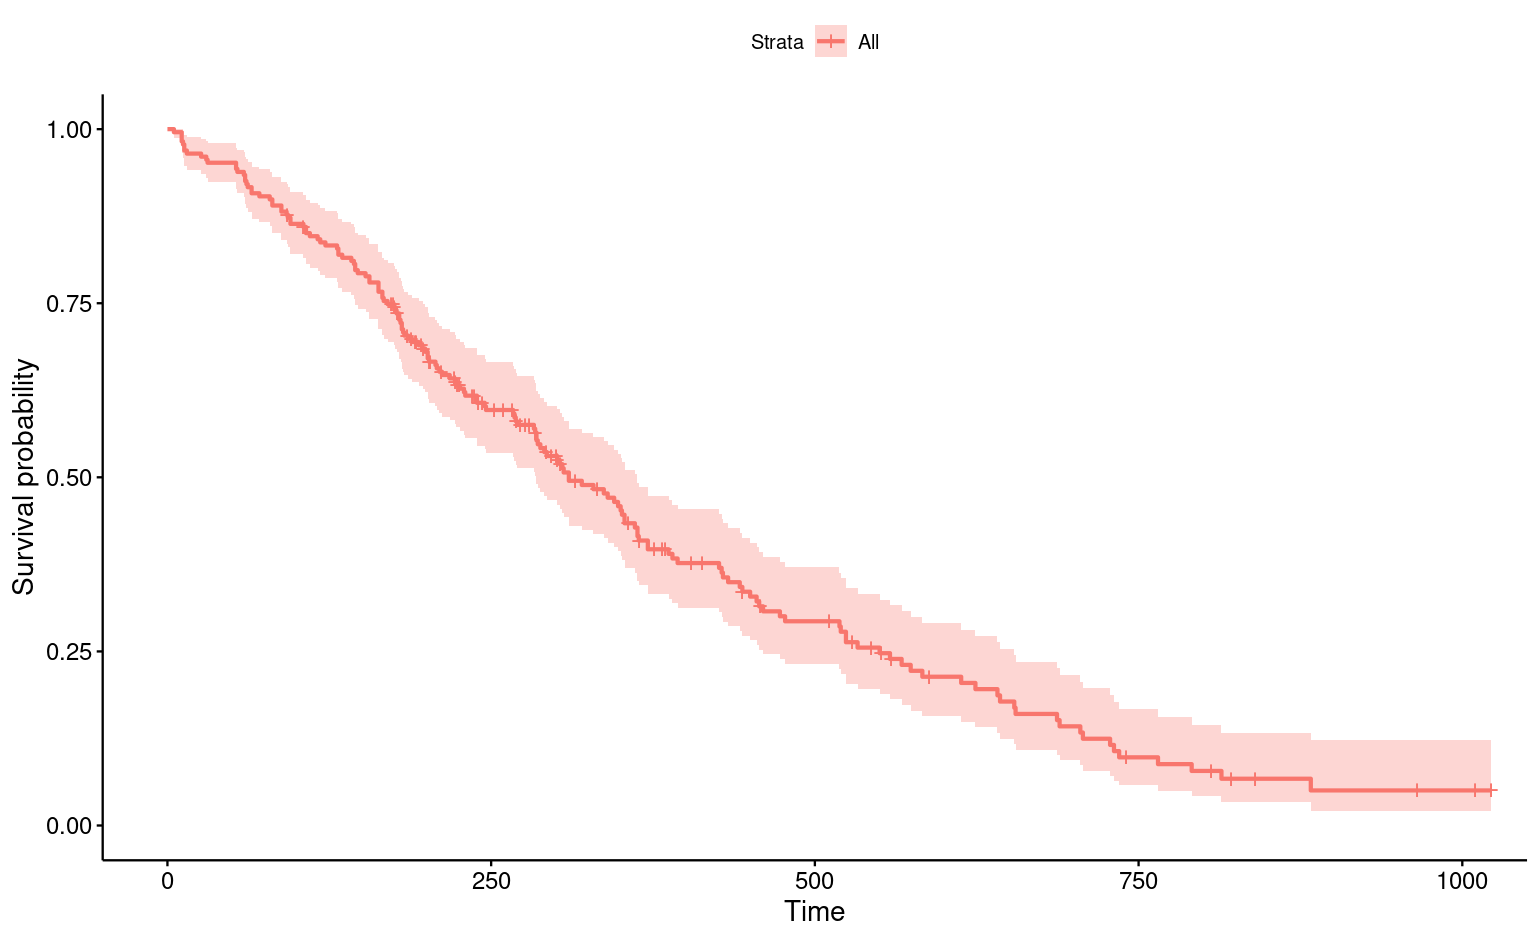
\includegraphics[scale=.33]{km_curve}
			\caption{The Kaplan-Meier estimate of the survivor function and the confidence limits.}
			\label{fig:km}
		\end{figure}
	\end{frame}
	
	\begin{frame}
		\frametitle{Kaplan-Meier estimate of the survivor function (cont.)}
		\framesubtitle{Hazard function}
		It's natural to estimate the hazard function as the death rate at a given time $t$ divided by the length of the time interval. Then the hazard function from $t_{ ( j ) }$ to $t_{ ( j + 1 ) }$ is estimated by 
		\[ \hat{ h }( t ) = \frac{ d_j }{ n_j \tau_j }, \]
		for $t_{ ( j ) } \leq t < t_{ ( j + 1 ) }$, where $\tau_j = t_{ ( j + 1 ) } - t_{ ( j ) }$.
		The estimated standard error is given by
		\[ \text{se}\{ \hat{ h }( t ) \} = \hat{ h }( t )\sqrt{ \frac{ n_j - d_j }{ n_j d_j } }. \]
	\end{frame}
	
	\begin{frame}
		\frametitle{Kaplan-Meier estimate of the survivor function (cont.)}
		\framesubtitle{Cumulative hazard function}
		Since $H( t ) = - \log S( t )$, the estimated cumulative hazard function is given by
		\[ \hat{ H }( t ) = - \sum_{ j = 1 }^{ k } \log \left( \frac{ n_j - d_j }{ n_j } \right). \]
	\end{frame}
	
	\begin{frame}
		\frametitle{Kaplan-Meier estimate of the survivor function (cont.)}
		\framesubtitle{Estimating the percentile}
		The estimated percentile is given by
		\[ \hat{ t }( p ) = \min\{ t_i | \hat{ S }( t_i ) < \frac{ p }{ 100 } \}, \]
		where $t_i$ is the observed survival time for the $i$th individual.
		The standard error of the percentiles is given by
		\[ \text{se}\{ \hat{ t }( p ) \} = \frac{ 1 }{ \hat{ f }\{ \hat{ t }( p ) \} } \text{se}[ \hat{ S }\{\hat{ t }( p )\} ], \]
		where $\hat{ f }\{ \hat{ t }( p ) \}$ is estimated density function at $\hat{ t }( p )$.
	\end{frame}
	
	\begin{frame}
		\frametitle{Kaplan-Meier estimate of the survivor function (cont.)}
		\framesubtitle{Estimating the density function}
		The estimated density function is given by
		\[ \hat{ f }\{ \hat{ t }( p ) \} = \frac{ \hat{ S }\{\hat{ u }( p )\} - \hat{ S }\{\hat{ l }( p ) \} }{ \hat{ l }( p ) - \hat{ u }( p ) }, \]
		where 
		\[ \hat{ u }( p ) = \max \left\{ t_{ ( j ) } | \hat{ S }( t_{ ( j ) } ) \geq 1 - \frac{ p }{ 100 } + \epsilon )  \right\}, \]
		and 
		\[ \hat{ l }( p ) = \max \left\{ t_{ ( j ) } | \hat{ S }( t_{ ( j ) } ) \leq 1 - \frac{ p }{ 100 } - \epsilon )  \right\}, \]
		for $j = 1, 2, \dots, r$, and small values of $\epsilon$. $\epsilon$ is usually taken as 0.05, however larger value will be required if $\hat{ u }( p ) = \hat{ l }( p )$.
	\end{frame}
	
	\begin{frame}[fragile]
		\frametitle{Kaplan-Meier estimate of the survivor function (cont.)}
		\framesubtitle{Comparison of two groups of survival data}
		It's straight forward to compare the estimated survival functions of the two groups.
	    \begin{Verbatim}[fontsize=\small]
## Compare the survivor functions of male and female
km_sex <- survfit( Surv( time, status ) ~ sex, data = lung )
## Generate graphs
ggsurvplot( km_sex,
            conf.int = TRUE, # add confidence intervals
            pval = TRUE, # show the p-value for the log-rank test
            risk.table = TRUE, # show a risk table below the plot
            legend.labs = c( "Male", "Female" ),
            legend.title = "Sex",
            palette = c("dodgerblue4", "orchid2"),
            title = "Kaplan-Meier Curve for Lung Cancer Survival",
            risk.table.height = .2 )
	    \end{Verbatim}
	\end{frame}
	
	\begin{frame}
		\frametitle{Kaplan-Meier estimate of the survivor function (cont.)}
		\framesubtitle{Comparison of two groups of survival data}
		
		\begin{figure}[H]
			\centering
			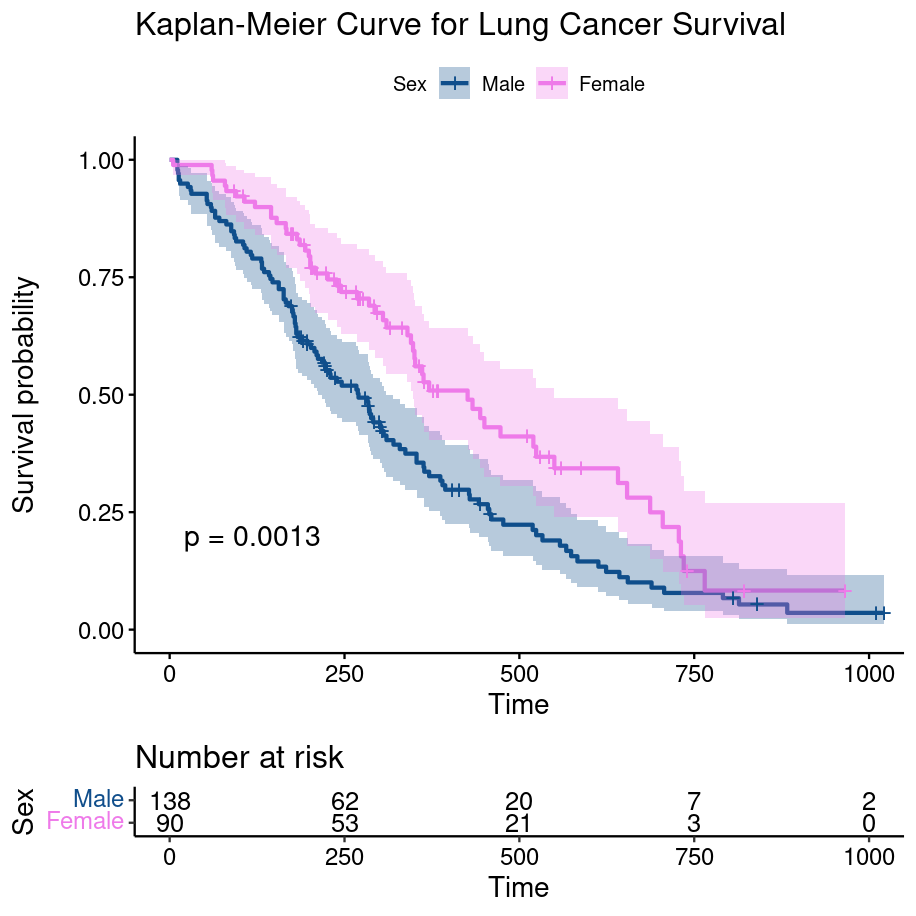
\includegraphics[scale=.4]{sex}
			\caption{The Kaplan-Meier estimate of the survivor function and the confidence limits for male and female.}
			\label{fig:sex}
		\end{figure}
	\end{frame}
	
	\begin{frame}
		\frametitle{Kaplan-Meier estimate of the survivor function (cont.)}
		\framesubtitle{The log-rank test}
		Non-parametric tests are used for testing the difference in the survivor functions between groups. Let $d_{ 1j }$ and $d_{ 2j }$ denote the number of death at time $t_{ ( j ) }$ in group 1 and 2, respectively. Let $n_{ 1j }$ and $n_{ 2j }$ denote the number of individuals at risk right before time $t_{ ( j ) }$ in group 1 and 2, respectively. Let $d_j = d_{ 1j } + d_{ 2j }$ and $n_j = n_{ 1j } + n_{ 2j }$.
		\begin{tabular}{cccc}
			\hline\hline
			Group & Number of  & Number of & Number at risk right \\
		
			& deaths at $t_{ ( j ) }$ & surviving over $t_{ ( j ) }$ & before $t_{ ( j ) }$ \\
			\hline
			1 & $d_{ 1j }$ & $n_{ 1j } - d_{ 1j }$ & $n_{ 1j }$ \\
			2  & $d_{ 2j }$ & $n_{ 2j } - d_{ 2j }$ & $n_{ 2j }$ \\
			\hline
			Total & $d_{ j }$ & $n_j - d_j$  & $n_j$ \\
			\hline\hline
		\end{tabular}
	Suppose the marginal totals in the table are fixed, then the four entries in the table is determined by the value of $d_{ 1j }$. If the survival is independent from group, then
	\[ d_{ 1j } \sim \text{Hypergeometric}( n_j, d_j, n_{ 1j } ).\]
	\end{frame}
	
	\begin{frame}
		\frametitle{Kaplan-Meier estimate of the survivor function (cont.)}
		\framesubtitle{The log-rank test}
		The mean of $d_{ 1j }$ is given by
		\[ e_{ 1j } = n_{ 1j } d_j / n_j. \]
		The variance of it is given by
		\[ v_{ 1j } = \frac{ n_{ 1j } n_{ 2j } d_j( n_j - d_j ) }{ n_j^2( n_j - 1 ) }.\]
		Let 
		\[ U_L = \sum_{ j = 1 }^{ r }( d_{ 1j } - e_{ 1j } ). \]
		Then 
		\[ \text{var}( U_L ) = \sum_{ j = 1 }^{ r } v_{ 1j } = V_L, \]
	\end{frame}
	
	\begin{frame}
		\frametitle{Kaplan-Meier estimate of the survivor function (cont.)}
		\framesubtitle{The log-rank test}
		It can be shown that 
		\[ \frac{ U_L }{ \sqrt{ V_L } } \sim N( 0, 1 ). \]
		Consequently,
		\[ \frac{ U_L^2 }{ V_L } \sim \chi_1^2. \]
	\end{frame}
	
	\begin{frame}
		\frametitle{Kaplan-Meier estimate of the survivor function (cont.)}
		\framesubtitle{The Wilcoxon test}
		If a weight $n_j$ is put on each $d_{ 1j } - e_{ 1j }$, then
		\[ U_W = \sum_{ j = 1 }^{ r } n_j( d_{ 1j } - e_{ 1j } ). \]
		The variance of $U_W$ is give by
		\[ V_W = \sum_{ j = 1 }^{ r } n_j^2 v_{ 1j } \]
		The Wilcoxon test statistic is 
		\[ W_W = U_W^2 / V_W, \]
		which follows $\chi^2_1$ when the null hypothesis is true.
	\end{frame}
	
	\begin{frame}
		\frametitle{Kaplan-Meier estimate of the survivor function (cont.)}
		\framesubtitle{Comparison of the two tests}
		The log-rank test is more appropriate when the hazard function of one group is proportional to that of the other group.
		
		If the hazard functions are proportional, then the survivor function don't cross one another.
	\end{frame}
	
	\begin{frame}[allowframebreaks]
		\begin{singlespace}
			\interlinepenalty=10000	% prevents bib items from splitting across pages
			\bibliography{survival}
			\bibliographystyle{apalike}
		\end{singlespace}
	\end{frame}
\end{document}